\documentclass[10pt]{article}  

%%%%%%%% PREÁMBULO %%%%%%%%%%%%
\usepackage[english]{babel} %Indica que escribiermos en español
\usepackage[utf8]{inputenc} %Indica qué codificación se está usando ISO-8859-1(latin1)  o utf8  
\usepackage{amsmath} % Comandos extras para matemáticas (cajas para ecuaciones,
% etc)
\usepackage{amssymb} % Simbolos matematicos (por lo tanto)
\usepackage{graphicx} % Incluir imágenes en LaTeX
\usepackage{color} % Para colorear texto
\usepackage{subfigure} % subfiguras
\usepackage{ulem}
\usepackage{amsmath}%%Usar ecuaciones
%%%%%%%%%%%%%CODIGO%%%%%%%%%%%%%%%%%%%%%%
\usepackage{listings} %Sirve para pegar codigo fuente de programas
\usepackage{caption}
\DeclareCaptionFont{white}{\color{white}}
\DeclareCaptionFormat{listing}{%
  \parbox{\textwidth}{\colorbox{gray}{\parbox{\textwidth}{#1#2#3}}\vskip-4pt}}
\captionsetup[lstlisting]{format=listing,labelfont=white,textfont=white}
\lstset{frame=ltrb,xleftmargin=\fboxsep,xrightmargin=-\fboxsep}
%%%%%%%%%%%%%CODIGO%%%%%%%%%%%%%%%%%%%%%%
\usepackage{float} %Podemos usar el especificador [H] en las figuras para que se
% queden donde queramos
\usepackage{capt-of} % Permite usar etiquetas fuera de elementos flotantes
% (etiquetas de figuras)
\usepackage{enumerate} % enumerados
\usepackage{sidecap} % Para poner el texto de las imágenes al lado
	\sidecaptionvpos{figure}{c} % Para que el texto se alinie al centro vertical
\usepackage{caption} % Para poder quitar numeracion de figuras
\usepackage{commath} % funcionalidades extras para diferenciales, integrales,
% etc (\od, \dif, etc)
\usepackage{cancel} % para cancelar expresiones (\cancelto{0}{x})
 
\usepackage{anysize} 					% Para personalizar el ancho de  los márgenes
\marginsize{2cm}{2cm}{2cm}{2cm} % Izquierda, derecha, arriba, abajo

\usepackage{appendix}

%Para la creación de tablas
\usepackage{array}
\newcolumntype{P}[1]{>{\centering\arraybackslash}p{#1}}
\newcolumntype{M}[1]{>{\centering\arraybackslash}m{#1}}
\usepackage{makecell}



%Para la creacion de cuadros de colores
\usepackage{tcolorbox}
\tcbuselibrary{listingsutf8}
% Cuadro numerado para ejemplos de cuadros de colores
\newtcolorbox[auto counter, number within=section]{example}[2][]
{colback=red!5!white,colframe=red!75!black,
fonttitle=\bfseries, title=Example~\thetcbcounter: #2,#1}

\newtcolorbox[auto counter, number within=section]{tip}[2][]
{colback=green!5!white,colframe=green!75!black,
fonttitle=\bfseries, title=Tip~\thetcbcounter: #2,#1}

% Para que las referencias sean hipervínculos a las figuras o ecuaciones y
% aparezcan en color
\usepackage[colorlinks=true,plainpages=true,citecolor=blue,linkcolor=blue]{hyperref}
%\usepackage{hyperref} 
% Para agregar encabezado y pie de página
\usepackage{fancyhdr} 
\pagestyle{fancy}
\fancyhf{}
\fancyhead[L]{\footnotesize VPLWVST} %encabezado izquierda
\fancyhead[R]{\footnotesize VP-TA}   % dereecha
\fancyfoot[R]{\footnotesize Tutorial A}  % Pie derecha
\fancyfoot[C]{\thepage}  % centro
\fancyfoot[L]{\footnotesize VisualPro: A Lightweight; Visual Scripting Tool}  %izquierda
\renewcommand{\footrulewidth}{0.4pt}


\usepackage{listings} % Para usar código fuente
\definecolor{dkgreen}{rgb}{0,0.6,0} % Definimos colores para usar en el código
\definecolor{gray}{rgb}{0.5,0.5,0.5} 
% configuración para el lenguaje que queramos utilizar
\lstset{basicstyle=\ttfamily,
   basicstyle=\ttfamily,
   keywordstyle=\color{blue},
   commentstyle=\color{red},
   stringstyle=\color{dkgreen},
   numberstyle=\tiny\color{gray},
   stepnumber=1,
   numbersep=10pt,
   backgroundcolor=\color{white},
   tabsize=4,
   showspaces=false,
   breaklines=true,
   showstringspaces=false}

\newcommand{\sen}{\operatorname{\sen}}	% Definimos el comando \sen para el seno
%en español
%%%%%%%% TERMINA PREÁMBULO %%%%%%%%%%%%

\begin{document}

%%%%%%%%%%%%%%%%%%%%%%%%%%%%%%%%%% PORTADA %%%%%%%%%%%%%%%%%%%%%%%%%%%%%%%%%%%%%%%%%%%%
																					%%%
\begin{center}																		%%%
\newcommand{\HRule}{\rule{\linewidth}{0.5mm}}									%%%\left
 																					%%%
\begin{minipage}{0.48\textwidth} \begin{flushleft}

\includegraphics[scale = 0.15]{Figures/Logo/UWTSD-Logo}
\end{flushleft}\end{minipage}
\begin{minipage}{0.48\textwidth} \begin{flushright}

\includegraphics[scale = 0.4]{Figures/Logo/VP-Logo-Large}
\end{flushright}\end{minipage}

													 								%%%
\vspace*{-1.5cm}								%%%
																					%%%	
\textsc{\huge Visual Pro\\ \vspace{5px} Tutorial A}\\[1.5cm]	

\textsc{\LARGE A beginners guide to Visual Scripting}\\[1.5cm]													%%%

\textsc{\Large VisualPro: A Lightweight; Visual Scripting Tool}\\[0.5cm]

    																				%%%
 			\vspace*{1cm}																		%%%
																					%%%
\HRule \\[0.4cm]																	%%%
{ \huge \bfseries Tutorial: Classes and Objects}\\[0.4cm]	%%%
 																					%%%
\HRule \\[1.5cm]																	%%%
 																				%%%
																					%%%
\begin{minipage}{0.4\textwidth}													%%%
\begin{flushleft} \large															
\textit{Authors:}\\
Edward Patch\\
Student Number: 1801492\\
\end{flushleft}																		%%%
\end{minipage}		
																%%%
\begin{minipage}{0.5\textwidth}		
\vspace{-0.6cm}											%%%
\begin{flushright} \large															%%%
\textit{Supervisor:} \\
Mike Dacey														%%%									
\end{flushright}																	%%%
\end{minipage}	
\vspace*{1cm}

\vspace{2cm} 																				
\begin{center}																					
{\large 16 February 2022}																	%%%
 			\end{center}												  						
\end{center}							 							
\newpage									
%%%%%%%%%%%%%%%%%%%% TERMINA PORTADA %%%%%%%%%%%%%%%%%%%%%%%%%%%%%%%%

\tableofcontents
\thispagestyle{fancy}

\newpage
\section{Learning Objectives}
The following learning objectives are as follows:
\begin{enumerate}
    \item Understanding the VisualPro application.
    \item Understanding the terminologies of classes, objects and methods.
    \item Writing several classes in a Visual Scripting environment.
\end{enumerate}


\newpage
\section{Introduction}
    \subsection{What is VisualPro?}
        VisualPro aims to create a lightweight Visual Scripting tool that encourages individuals to the development field. VisualPro enables users to create code structures to help develop ideas into reality. \\\textbf{Note:} VisualPro does not have logical programming tools in its current implementation.

    \subsection{What will the tutorial cover?}
        The tutorial covers VisualPro Environment of how to use the software, found in section~\ref{sec:vp-env}, page~\pageref{sec:vp-env} and terminology found in section~\ref{sec:terminology}, page~\pageref{sec:terminology}.
        The tutorial teaches the basics of Object-Oriented and how to implement the structure within VisualPro, found in section~\ref{sec:object-orientation}, page~\pageref{sec:object-orientation}.
        
        \begin{example}{Object-Oriented Languages (or) Languages with Object-Oriented Features}
            C++, C\# and Java. To view other object-oriented languages,\\~\href{https://worddisk.com/wiki/List_of_object-oriented_programming_languages/}{WordDisk - Languages with object-oriented features}~\cite{word_disk_list_2018}.
        \end{example}

    \begin{tip}{Important:}
        Make sure to work through the survey when working through the survey. A description of each section of the survey, similar to `Refer to Tutorial | Exercise:' helps pinpoint which section relates to the exercise found within the tutorial.
    \end{tip}

\section{VisualPro Environment}
\label{sec:vp-env}
    \subsection{Download VisualPro}
        Download the~\href{https://github.com/ShinkuKira21/VisualPro-FinalProject/releases/tag/VP-V0.06A}{VisualPro V0.06a}~\cite{patch_visualpro_2022}. If download does not work, scroll down to the references and look for cite \textit{2}.

        \begin{tip}{Tip:}
            VisualPro can run without extraction. However, extraction ensures no problems when running the application.
        \end{tip}
    \subsection{Features}
        VisualPro offers a few features such as:
        \begin{itemize}
            \item Classes, Functions and Arguments, and Variables.
            \item Saving in Multiple Languages.
            \item Drag and Drop Elements and Text Areas.
            \item Property Windows to Control Arguments and Relationships.
        \end{itemize}

    \subsection{Known Bugs}
    \label{subsec:ve-knownbugs}
        A couple of bugs include:-
        \begin{itemize}
            \item Arguments for functions are not currently available.
            \item Deleting containers does not mathematically reset the following location or move existing containers backwards.
            \item A recent bug found from a unit test shows that sometimes the ReplaceString function within the backend fails. This problem causes the code to render without details. 
            \item \textbf{Update:} A workaround for the ReplaceString bug is in place. However, any empty text fields (even if the language does not require the text box) will cause the code to not render in full detail.
        \end{itemize}

    \subsection{Saving Progress}
        After completing a tutorial, select the language and press save.

        \begin{tip}{Compatibility}
            As mentioned previously, not all languages support object-orientation. If a language is not compatible with a particular keyword, the code generator will ignore the selected syntax object.

            \textbf{Example Language:} C is not supported.
        \end{tip}

\section{Terminology}
\label{sec:terminology}
    \subsection{What is a Class?}
        A class enables developers to containerise code that is referenced later as objects. Java language enables the demonstration of a typical Class declaration in an Object-Oriented Programming (OOP) environment. \textbf{Note:} The default access modifier of a Class is \textit{private}.

        \begin{example}{Code Example - C\# and Java}
            An example syntax of declaring a class in C\# and Java languages:-
            \begin{lstlisting}[language=java]
                public class Name { 
                    protected void Method_A() {}
                    public void Method_B() {}
                    private void Method_C() {}
                }
            \end{lstlisting}

            Within languages similar to C\# and Java, member tags enable scope-protection to classes, methods and variables with different purposes. The code snippet displays that the declaration of members, public, private, and protected members align with the class or method declaration. However, only one \textit{public} Class can exist within the Java language if the file name and extension is \textbf{ClassName.java}. Whereas in C\#, multiple \textit{public} Classes can exist. To understand classes and modifiers within C\#, look at~\href{https://docs.microsoft.com/en-us/dotnet/csharp/fundamentals/types/classes}{Classes in the C\# Language}-~\cite{bill_wagner_classes_2021}. 
        \end{example} 

        \begin{example}{Code Example - C++}
            \begin{lstlisting}[language=c++]
                class Name { 
                    protected:
                        void Method() {}
                    public:
                        void Method() {}
                    private: 
                        void Method() {}
                };
            \end{lstlisting}
            C++ language uses member colon style with a new line. To understand C++ classes and modifers, look at~\href{https://www.cplusplus.com/doc/tutorial/classes/}{Classes in C++ Language}~\cite{cpluspluscom_classes_nodate}\\
            \textbf{Note:} - the modifiers of protected, public and private members mean the same as the previous example.
        \end{example}

    \newpage
    \subsection{What is a Method?}
        Methods belong within a class that interacts with neighbour methods and variables, child class methods and variables or object methods and variables (dependent on the access modifier).
        
        Unlike Class containers, Methods execute a `script' that \textbf{can} communicate with inherited Variables and Members, usually using the \textit{this} (C++, C\# or Java) or \textit{self} (Python) keyword dependent on the programming language.

        \begin{tip}{Documentation Tip}
            When using a programming language, it is important not to remember every language's syntax. As programming languages are the same, `not all size fits the one' tool, sometimes it is beneficial to try different languages to fix the same problem to see many different methods available. After learning the generic tools, progressing from one language to another becomes a relaxed and speedy experience. Refer to the programming language documentation for any uncertainties.
        \end{tip}

    \subsection{What is an Object?}
        When referencing a Class in another instance, it is important to remember that this is called an Object. Two examples of objects demonstrates the meaning, with a reference of what an Object is to enable further study on this terminology.

        \begin{example}{Object Demonstration (C\# and Java Language)}

            \textbf{Java:}
            \begin{lstlisting}[language=java]
                class Car {
                    public int x;
                    public void AddToX(int x) {
                        this.x += x;
                    }
                }

                class Program { 
                    public static void Main(String[] args) {
                        // Object Car 
                        Car mustang = new Car();

                        mustang.x = 1;
                        mustang.AddToX(10);
                        System.out.println(mustang.x);
                    }
                }
            \end{lstlisting}

            \textbf{C\#:}
            \begin{lstlisting}[language=java]
                class Car {
                    public int x;
                    public void AddToX(int x) {
                        this.x += x;
                    }
                }

                class Program { 
                    static void Main(string[] args) {
                        // Object Car 
                        Car mustang = new Car();
                
                        mustang.x = 1;
                        mustang.AddToX(10);
                        Console.WriteLine(mustang.x);
                    }
                }
            \end{lstlisting}
        \end{example}

        \newpage
        An example of an object within C++:-
        \begin{example}{C++ Object}
            \begin{lstlisting}[language=c++]
                class Car {
                    public:
                        int x;
                        void AddToX(int x)
                        { this->x += x; }                   }
                };

                void main(int argc, char* argv)
                {
                    Car mustang;
                    
                    mustang.x = 1;
                    mustang.AddToX(10);
                    
                    std::cout << mustang.x;

                    return 0;
                }
            \end{lstlisting}

            \textbf{Important:} Notice how the `main' function is not within a class wrapper? This fact is because C++ is a Functional Programming style and OOP style. \textit{More on this in Tutorial B.}
        \end{example}

\section{Object-Orientation}
\label{sec:object-orientation}
    \subsection{Exercise: Understanding the Basics}
        VisualPro offers three structures, Class, Functions and Variables. This tutorial focuses on the Class structure, and the following exercises aim to provide knowledge of how Classes work in two different OOP languages.

        On the left of VisualPro is the selection of structure tools. These are draggable objects only. These tools can drop onto the Work Area panel on the right side of the VisualPro window. The containers that appear within the workplace enable three text areas, Properties and Child Work Area, to configure the Class, Function or Variables for more advanced setup. Example images may help draw a picture of the sections mentioned.

        \begin{tip}{Evidencing}
            \textbf{Necessary:} Make sure to copy each exercise code to the survey when asked. A reference of the survey question helps find the corresponding survey question to paste the final code.
        \end{tip}

    \newpage
    \subsection{Exercise: Initial Partipation}
        Within the VisualPro survey, did you answer `Yes' to the first question? If so, continue this task. Otherwise, skip this exercise.

        Drag and drop a few classes, functions (methods) or variables, and test the software by removing and adding new items. Answer the questions based on the comparison of the Programming Planner and provide details on the experience. Feel free to express any views on the video feed. Beware of any bugs mentioned within the Known Bugs, section~\ref{subsec:ve-knownbugs}, page~\pageref{subsec:ve-knownbugs}.

    \newpage
    \subsection{Exercise: Creating a Class}
        To create a Class inside of VisualPro, drag and drop the \textit{Class} within the \textit{Outline Tool} area inside the \textit{Work Area} panel. As mentioned previously, this will create a container inside the Work Area panel.

        \textbf{Tasks:-}
        \begin{enumerate}
            \item Name the Class, `World'. A class does not require a Member, and Data-Type should remain empty.
            \item After creating the Class, save the file with the language C++.
        \end{enumerate}
        Name the Class, `World'. A class does not require a Member and Data-Type should remain empty. Once the Class is created, save the file with the language C++ and copy the file content.

        \textbf{Did it look like this visually?:-}
            \begin{figure}[h]
                \centering
                {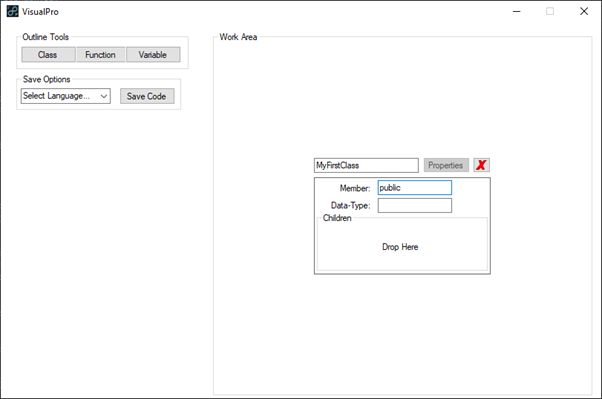
\includegraphics[scale=0.75]{Figures/Exercises/SecB-1.png}}
                \caption{VisualPro - Exercise A}
                \label{fig:vp-eA}
            \end{figure}

        \textbf{Expected Code Generation:-}\\
        The code should look similar to this:
        \begin{example}{C++ Class}
            \begin{lstlisting}[language=c++]
                class World {

                };
            \end{lstlisting}
        \end{example}

        \begin{example}{C\# Class}
            \begin{lstlisting}[language=java]
                public class World {

                }
            \end{lstlisting}
        \end{example}
    \newpage
    \subsection{Exercise: Animal Types}
        Remember that a Class is a template containing variables and methods related to how to shape the functionality and data of what the object can carry? For this example, the Class will contain three types of animals: Reptiles, Mammals and Amphibians.
        
        % Cold Blooded, Warm Blooded and Aqua
        \textbf{Survey Question:-} What main methods variables separate Reptiles, Mammals and Amphibians from one another?

        Now, create three classes of the mentioned types. After creating the classes, save the file with C\# or C++, as C does not support OOP. Submit your code to:-

        \textbf{Did it look like this visually?:-} 
        \begin{figure}[h]
            \centering
            {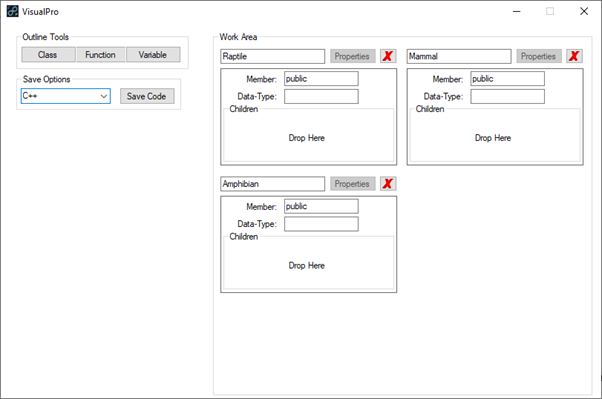
\includegraphics[scale=0.75]{Figures/Exercises/SecC-1.png}}
            \caption{VisualPro - Exercise B}
            \label{fig:vp-eB}
        \end{figure}

        \textbf{Expected Code Generation:-}\\
        The code should look similar to this:
        \begin{example}{C++ Classes}
            \begin{lstlisting}[language=c++]
                class Reptile {

                };

                class Mammals {

                };

                class Amphibian {

                };
            \end{lstlisting}
        \end{example}

        \begin{example}{C\# Classes}
            \begin{lstlisting}[language=java]
                public class Reptile {

                }

                public class Mammal {

                }

                public class Amphibian {

                }
            \end{lstlisting}
        \end{example}

    \newpage
    \subsection{Exercise: Vehicle Components}
    Well done! Classes are now a tool that is no longer scary. However, learning requires do-overs. However, adding methods or variables is vital to learning how to declare variables and methods in a class. \textit{(VisualPro only supports one method or variable at the present moment)}. Now let us try this example.

    A car has a various components such as body, engine and wheels to help the car work correctly. \textbf{Challenge:} Create two components of a car and give a descriptive method or variable (to do this drag a function/variable on the child work area.)

    \textbf{An example is given:-}
    \begin{figure}[h]
        \centering
        {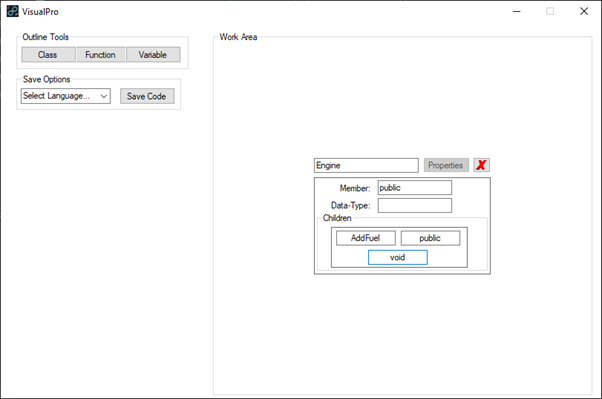
\includegraphics[scale=0.75]{Figures/Exercises/SecD-1.png}}
        \caption{VisualPro - Exercise C}
        \label{fig:vp-eC}
    \end{figure}

    \begin{tip}{Data-Types}
        A datatype on a function/method acts as a return type. A function can return data to get the required data—more on this in Tutorial B. For now, type (void) as the datatype.

        However, if it is a variable, try thinking about the variable's type of data. For example, if it holds a whole number, use an int (for integer); if it is text, then type string or if a decimal value comes to mind, try float—more on this on Tutorial B. 
    \end{tip}

    \subsection{Exercise: Try It Yourself (TIY)}
        Feel free to explore the classes with methods and variables, and submit your code.\\
        \textbf{Some examples:-} A computer class, a planet class or a calculator class.
\section{Keywords}
\label{sec:keywords}
    \begin{itemize}
        \item OOP - Object-Orinted Programming.
    \end{itemize}

%%%%%%% References %%%%%%%%
\clearpage
\nocite{*}
\small{\bibliographystyle{IEEEtran}
\bibliography{ref}}
%%%%%%% References %%%%%%%%      
\end{document}